\documentclass[]{book}
\usepackage{lmodern}
\usepackage{amssymb,amsmath}
\usepackage{ifxetex,ifluatex}
\usepackage{fixltx2e} % provides \textsubscript
\ifnum 0\ifxetex 1\fi\ifluatex 1\fi=0 % if pdftex
  \usepackage[T1]{fontenc}
  \usepackage[utf8]{inputenc}
\else % if luatex or xelatex
  \ifxetex
    \usepackage{mathspec}
  \else
    \usepackage{fontspec}
  \fi
  \defaultfontfeatures{Ligatures=TeX,Scale=MatchLowercase}
\fi
% use upquote if available, for straight quotes in verbatim environments
\IfFileExists{upquote.sty}{\usepackage{upquote}}{}
% use microtype if available
\IfFileExists{microtype.sty}{%
\usepackage{microtype}
\UseMicrotypeSet[protrusion]{basicmath} % disable protrusion for tt fonts
}{}
\usepackage{hyperref}
\hypersetup{unicode=true,
            pdftitle={Notes on Maple for Calculus II},
            pdfauthor={Fei Ye},
            pdfborder={0 0 0},
            breaklinks=true}
\urlstyle{same}  % don't use monospace font for urls
\usepackage{natbib}
\bibliographystyle{plainnat}
\usepackage{longtable,booktabs}
\usepackage{graphicx,grffile}
\makeatletter
\def\maxwidth{\ifdim\Gin@nat@width>\linewidth\linewidth\else\Gin@nat@width\fi}
\def\maxheight{\ifdim\Gin@nat@height>\textheight\textheight\else\Gin@nat@height\fi}
\makeatother
% Scale images if necessary, so that they will not overflow the page
% margins by default, and it is still possible to overwrite the defaults
% using explicit options in \includegraphics[width, height, ...]{}
\setkeys{Gin}{width=\maxwidth,height=\maxheight,keepaspectratio}
\IfFileExists{parskip.sty}{%
\usepackage{parskip}
}{% else
\setlength{\parindent}{0pt}
\setlength{\parskip}{6pt plus 2pt minus 1pt}
}
\setlength{\emergencystretch}{3em}  % prevent overfull lines
\providecommand{\tightlist}{%
  \setlength{\itemsep}{0pt}\setlength{\parskip}{0pt}}
\setcounter{secnumdepth}{5}
% Redefines (sub)paragraphs to behave more like sections
\ifx\paragraph\undefined\else
\let\oldparagraph\paragraph
\renewcommand{\paragraph}[1]{\oldparagraph{#1}\mbox{}}
\fi
\ifx\subparagraph\undefined\else
\let\oldsubparagraph\subparagraph
\renewcommand{\subparagraph}[1]{\oldsubparagraph{#1}\mbox{}}
\fi

%%% Use protect on footnotes to avoid problems with footnotes in titles
\let\rmarkdownfootnote\footnote%
\def\footnote{\protect\rmarkdownfootnote}

%%% Change title format to be more compact
\usepackage{titling}

% Create subtitle command for use in maketitle
\providecommand{\subtitle}[1]{
  \posttitle{
    \begin{center}\large#1\end{center}
    }
}

\setlength{\droptitle}{-2em}

  \title{Notes on Maple for Calculus II}
    \pretitle{\vspace{\droptitle}\centering\huge}
  \posttitle{\par}
    \author{Fei Ye}
    \preauthor{\centering\large\emph}
  \postauthor{\par}
      \predate{\centering\large\emph}
  \postdate{\par}
    \date{2019-07-15}

\usepackage{booktabs}

\usepackage{amsthm}
\newtheorem{theorem}{Theorem}[chapter]
\newtheorem{lemma}{Lemma}[chapter]
\newtheorem{corollary}{Corollary}[chapter]
\newtheorem{proposition}{Proposition}[chapter]
\newtheorem{conjecture}{Conjecture}[chapter]
\theoremstyle{definition}
\newtheorem{definition}{Definition}[chapter]
\theoremstyle{definition}
\newtheorem{example}{Example}[chapter]
\theoremstyle{definition}
\newtheorem{exercise}{Exercise}[chapter]
\theoremstyle{remark}
\newtheorem*{remark}{Remark}
\newtheorem*{solution}{Solution}
\let\BeginKnitrBlock\begin \let\EndKnitrBlock\end
\begin{document}
\maketitle

{
\setcounter{tocdepth}{1}
\tableofcontents
}
\chapter*{Introduction}\label{introduction}
\addcontentsline{toc}{chapter}{Introduction}

This is a book written for labs for Calculus II.

\section*{What should I do after I opened
Maple}\label{what-should-i-do-after-i-opened-maple}
\addcontentsline{toc}{section}{What should I do after I opened Maple}

Once you opened Maple, you will see the following Maple Start document.
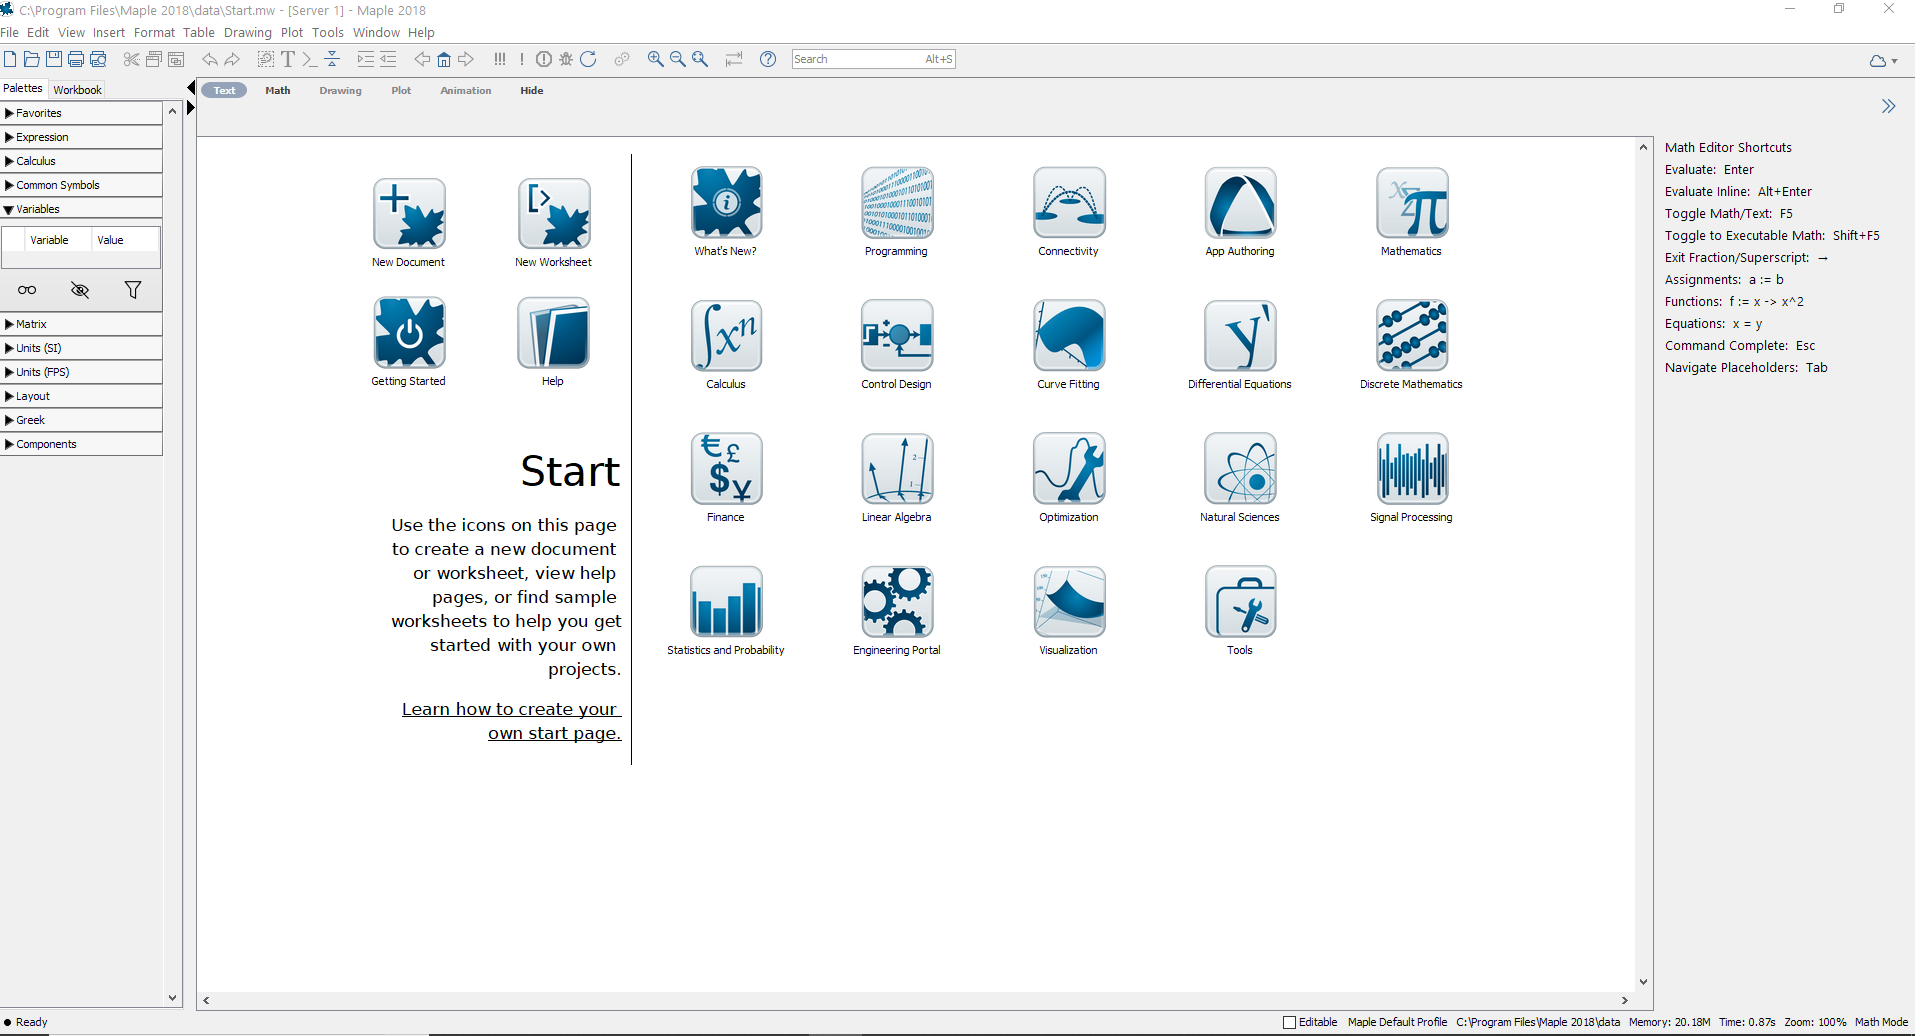
\includegraphics{figs/Maple-Start.png}

\begin{itemize}
\tightlist
\item
  If you already know what you want to do, then you may open a new
  document by clicking \texttt{New\ Document} icon in the start
  document. The following shows what an new (empty document) looks like.
\end{itemize}

\begin{figure}
\centering
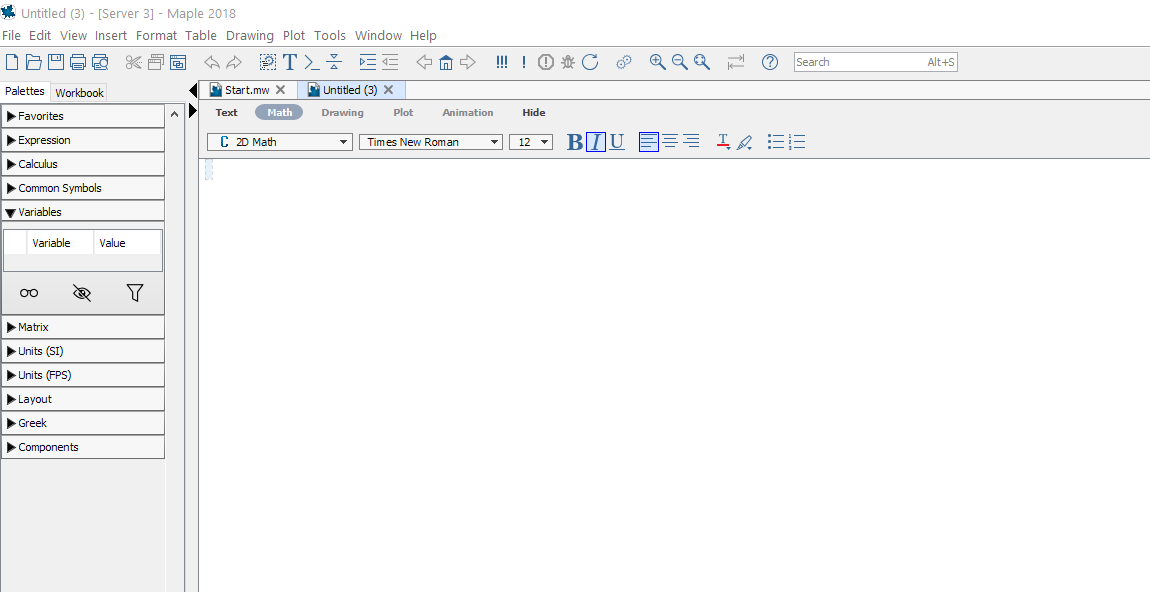
\includegraphics{figs/Maple-New-Doc.png}
\caption{}
\end{figure}

In this new document you may type in text under \texttt{Text} mode or
evaluat a Maple syntax in the \texttt{Math} mode. (See the following
picture).

\begin{figure}
\centering
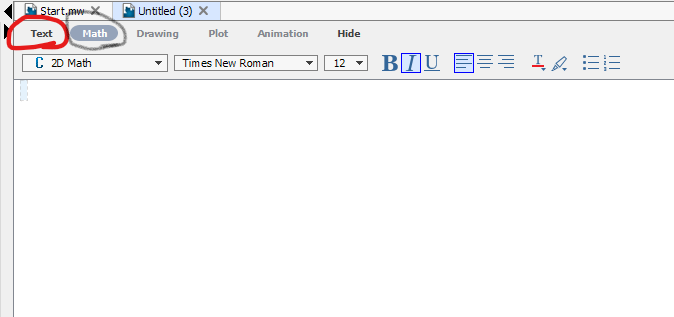
\includegraphics{figs/Text-Math-Mode.png}
\caption{}
\end{figure}

\begin{itemize}
\item
  If you want to explore some featured sample documents, you may go to
  \texttt{Start.mw} document and click on different icons to open a new
  document.
\item
  You may alway reopen the start page by click the home icon to reopen
  the start page.
\end{itemize}

\begin{figure}
\centering
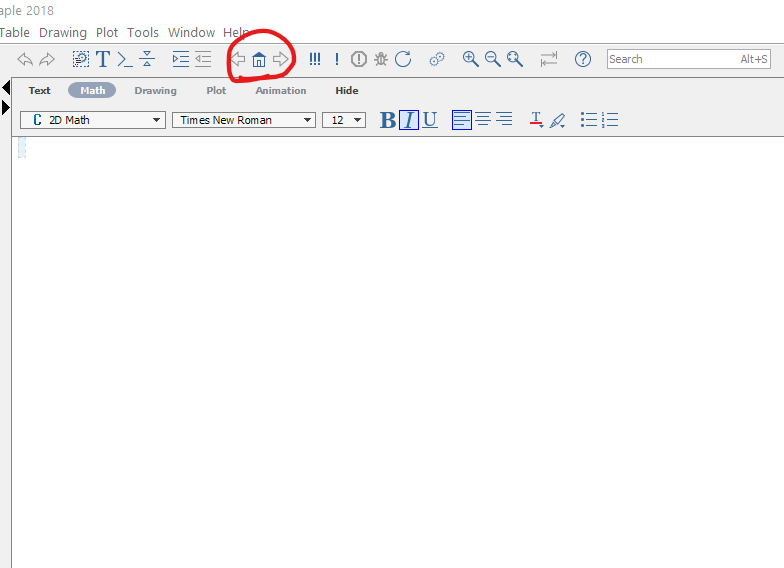
\includegraphics{figs/Home-reopen-start-page.png}
\caption{}
\end{figure}

\begin{itemize}
\tightlist
\item
  For Caculus, the most useful document is \texttt{Calculus}.
\end{itemize}

\begin{figure}
\centering
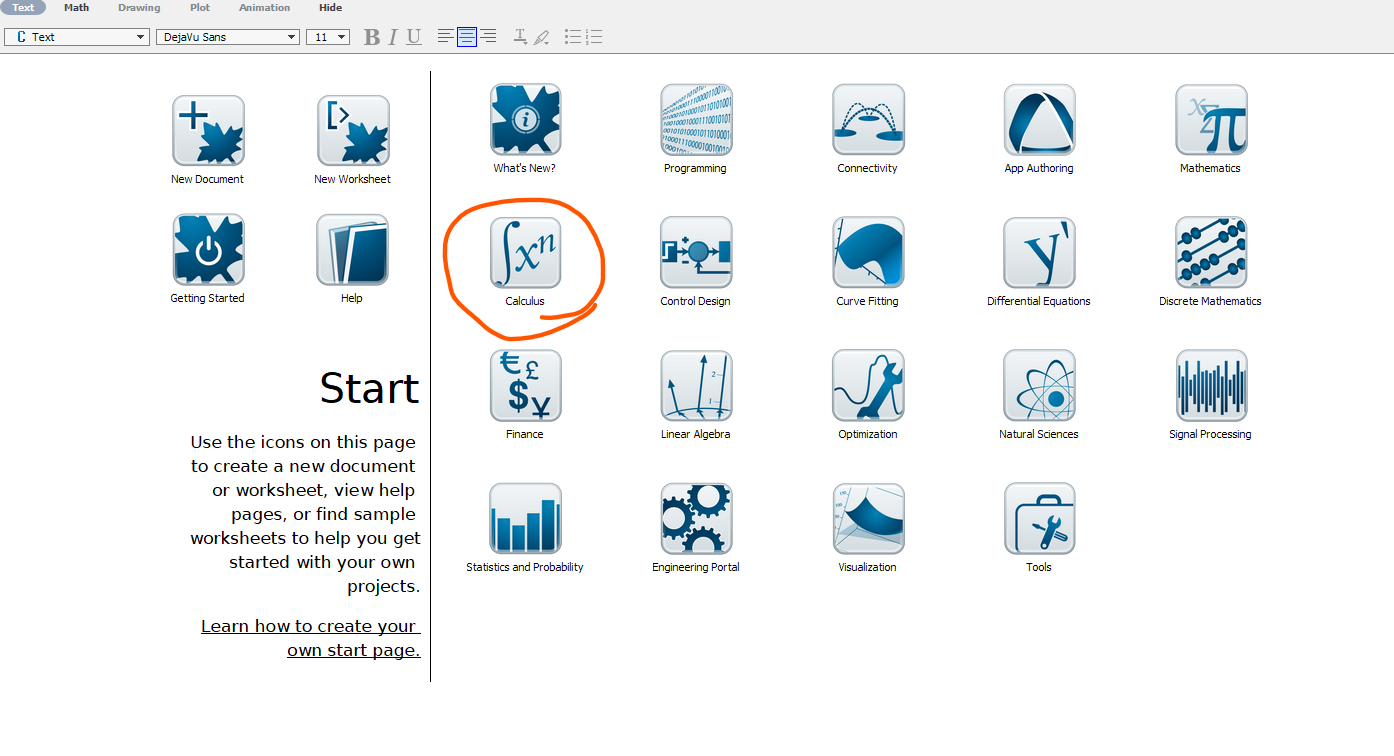
\includegraphics{figs/Start-Page-Calculus.png}
\caption{}
\end{figure}

If you click the \texttt{Calculus} icon on the Start page and click
\texttt{OK}, you will see the following document.

\begin{figure}
\centering
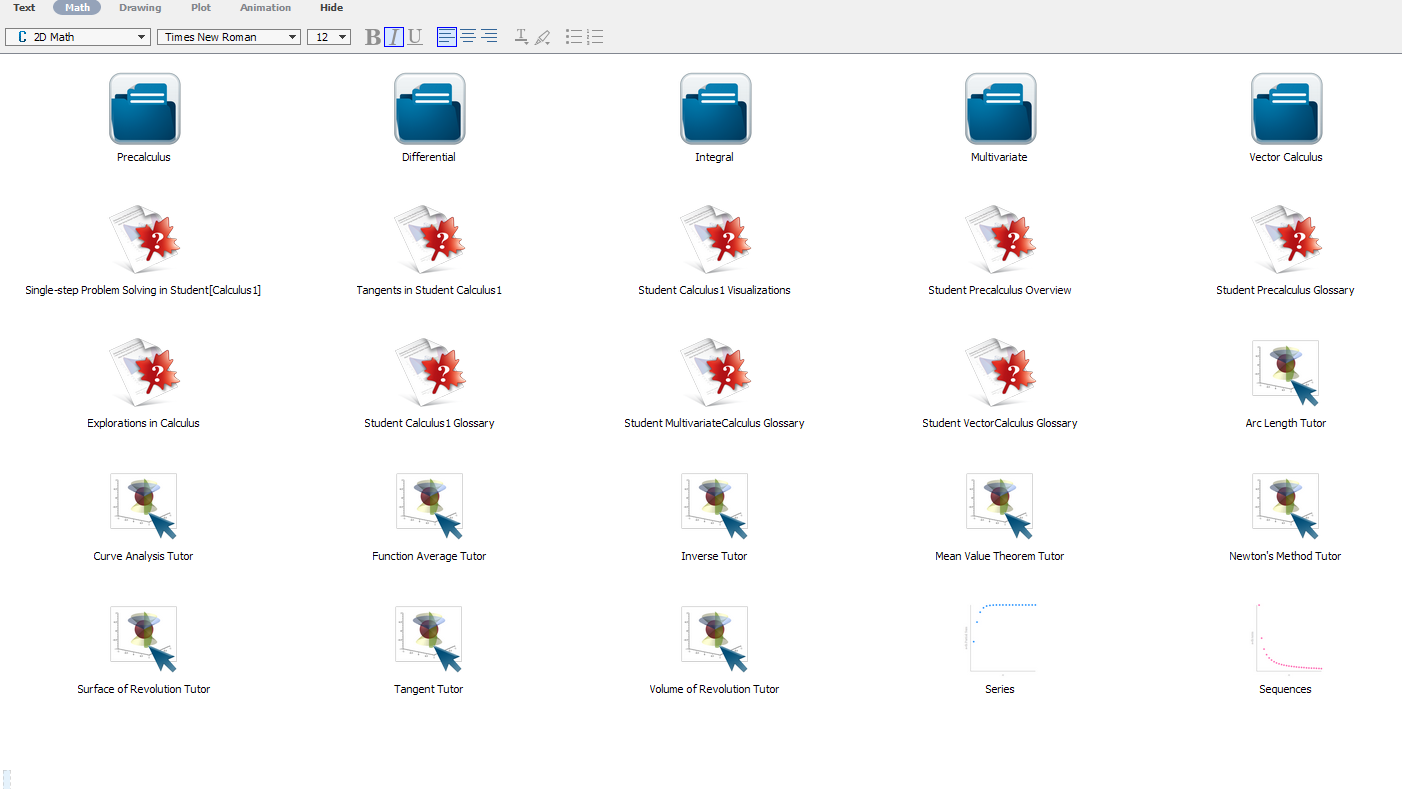
\includegraphics{figs/Calculus-Doc.png}
\caption{}
\end{figure}

\chapter{Volume of Revolution}\label{volume-of-revolution}

In terms of definite integrals, the volume of a solid obtained by
rotating a region about the \(x\)-axis can be calculated by
\[\int_a^b \pi (r_1(x)^2 - r_2(x)^2) \mathrm{d} x \qquad \text{disk/washer method},\]
or
\[\int_a^b 2\pi r(y) h(y) \mathrm{d} y \qquad \text{shell method method},\]

where \(r_1(x)\), \(r_2(x)\) and \(r(x)\) represents the radius and
\(h(x)\) represents the height of a cylindrical shell.

In practice, it's better to recognize the shape of a cross section, find
the volume of a slice of the solid and then set up the integral.

In the following, you will see some tools/commands from Maple which are
very helpful to calculate the volume of a solid.

In Maple, the following command, supported by the package
\texttt{Student{[}Calculus1{]}}, can be used to get the graph, the
integral and the volume of the solid obtained by rotation the region
bounded by \(f(x)\), \(g(x)\), \(x=a\) and \(x=b\).

\begin{verbatim}
VolumeOfRevolution(f(x), g(x), x = a..b, opts)
\end{verbatim}

To learn what options does the command \texttt{VolumeOfRevolution} have,
you may type

\begin{verbatim}
?VolumeOfRevolution
\end{verbatim}

in the Math mode and hit enter. You will see the help page.

\begin{figure}
\centering
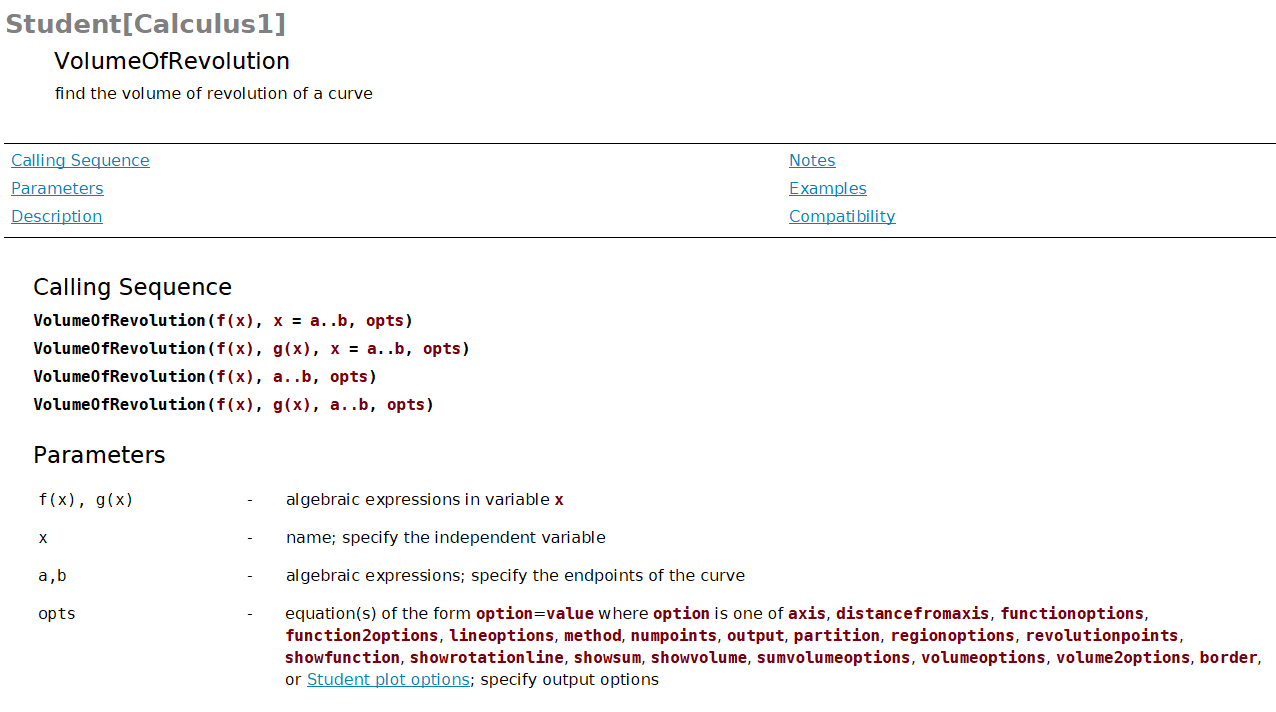
\includegraphics{figs/VolOfRev-help-page.png}
\caption{}
\end{figure}

\BeginKnitrBlock{example}
\protect\hypertarget{exm:unnamed-chunk-1}{}{\label{exm:unnamed-chunk-1}
}Show the solid obtained by rotating the region bounded by \(y=x^2\) and
\(y=x\) about \(y\)-axis. Set up an integral for the volume. Find the
volume.
\EndKnitrBlock{example}

\BeginKnitrBlock{solution}
\iffalse{} {Solution. } \fi{}

\chapter{Load the package}\label{load-the-package}

\begin{verbatim}
with(Student[Calculus1])
\end{verbatim}

\chapter{Show the solid}\label{show-the-solid}

\begin{verbatim}
VolumeOfRevolution(x^2, x, x = 0 .. 1, axis = vertical, output = plot)
\end{verbatim}

\chapter{Set up an integral}\label{set-up-an-integral}

\begin{verbatim}
VolumeOfRevolution(x^2, x, x = 0 .. 1, axis = vertical, output = integral)
\end{verbatim}

\chapter{Find the volume}\label{find-the-volume}

\begin{verbatim}
VolumeOfRevolution(x^2, x, x = 0 .. 1, axis = vertical, output = value)
\end{verbatim}

The outputs in Maple can be seen in the following picture

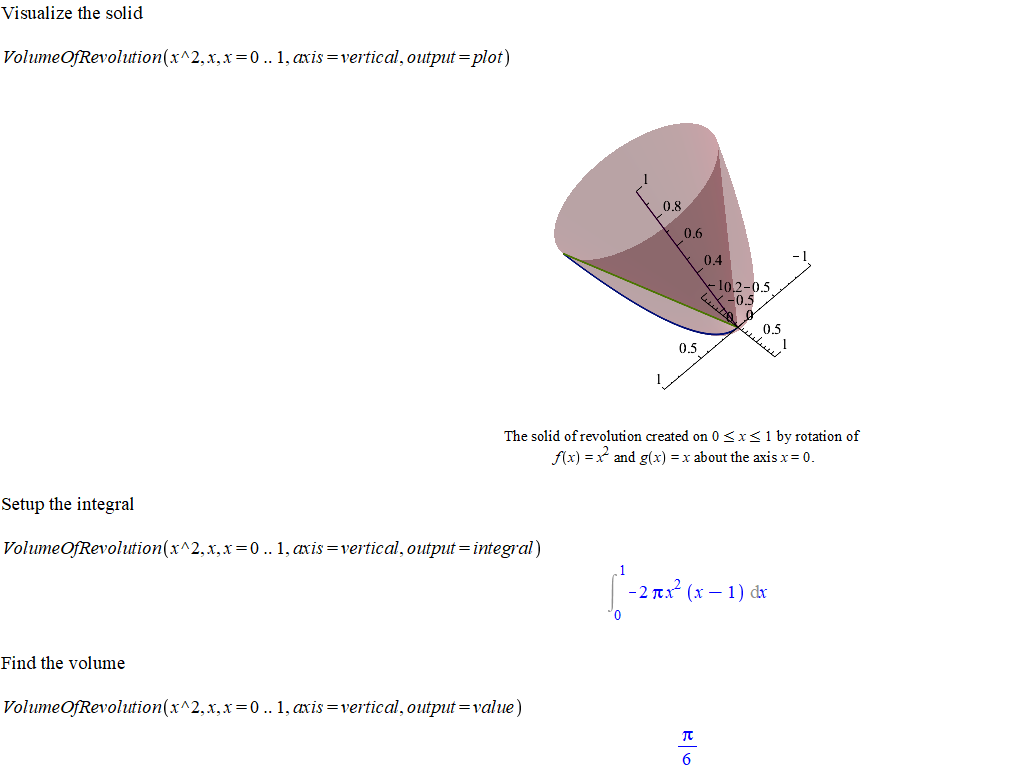
\includegraphics{figs/VolOfRev-Example1.png}
\EndKnitrBlock{solution}

\BeginKnitrBlock{remark}
\iffalse{} {Remark. } \fi{}1. If you change the function to
\texttt{VolumeOfRevolutionTutor}, you will see an interactive popup
windows which does exactly the same thing.

\begin{enumerate}
\def\labelenumi{\arabic{enumi}.}
\setcounter{enumi}{1}
\item
  If the rotation axis is not an axis of the coordinate system, you need
  add the option \texttt{distancefromaxis\ =\ numeric} into the
  function. For example, if in the above example, the rotation is about
  \(y=-2\), then the Maple command should be the following

\begin{verbatim}
VolumeOfRevolution(x^2, x, x = 0 .. 1, axis = vertical, distancefromaxis = -2, output = integral)
\end{verbatim}
\end{enumerate}
\EndKnitrBlock{remark}

\BeginKnitrBlock{exercise}
\protect\hypertarget{exr:unnamed-chunk-4}{}{\label{exr:unnamed-chunk-4}
}Find the volume of the solid obtained by rotating the region bounded by
\(y=x^3\), \(x=0\), \(y=1\) about \(y\)-axis
\EndKnitrBlock{exercise}

\BeginKnitrBlock{exercise}
\protect\hypertarget{exr:unnamed-chunk-5}{}{\label{exr:unnamed-chunk-5}
}Find the volume of the solid obtained by rotating the region bounded by
\(y=x^3\), \(y=0\), \(x=1\) about (a) \(y=0\), and (b) \(x=2\).
\EndKnitrBlock{exercise}

\chapter{Inverse Functions}\label{inverse-functions}

Maple package \texttt{Student{[}Calculus1{]}} provides the following
command

\begin{verbatim}
InversePlot(f(x), x = a..b);
\end{verbatim}

which graphs the original function \(f(x)\) and the inverse function
\(f^{-1}(x)\) together over the interval \([a, b]\).

You will see clearly that the graphs of a function and its inverse are
symmetric with respect to the line \(y=x\).

\BeginKnitrBlock{example}
\protect\hypertarget{exm:unnamed-chunk-1}{}{\label{exm:unnamed-chunk-1} }

\begin{enumerate}
\def\labelenumi{\arabic{enumi}.}
\item
  Graph the function \(f(x)=x^3-2\), its inverse function, and the line
  \(y=x\) over the interval \([-2,2]\).
\item
  Find the inverse function.
\end{enumerate}
\EndKnitrBlock{example}

\BeginKnitrBlock{solution}
\iffalse{} {Solution. } \fi{} One way to plot the function and its
inverse together is to use the following command which is supported by
the package \texttt{Student{[}Calculus1{]}}.

\begin{verbatim}
  InversePlot(x^3-3, x = -2 .. 2)
\end{verbatim}

Here is the output in Maple

\begin{figure}
\centering
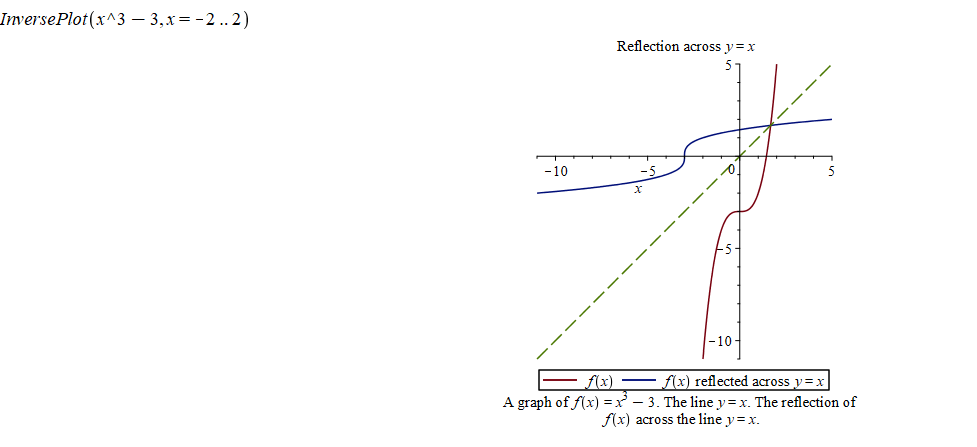
\includegraphics{figs/InversePlot1.png}
\caption{Graph of a pair of functions inverse to each other}
\end{figure}

Another way to plot the function \(f\) and its inverse \(g\) together
uses the \texttt{plot} function.

\begin{verbatim}
  plot([f(x), g(x), x], x = -2 .. 4, y = -5 .. 5, color = [red, black, blue])
\end{verbatim}

To find the inverse function, we replace \(f(x)\) by \(y\), then switch
\(x\) and \(y\), and solve for \(y\). In Maple, you may use the command
\texttt{solve(equation/inequality,\ variable)} to solve an equation or
an inequality (even system of equations/inequalities).

In this example, we may find the inverse function by type in the
following command. Note I have switch \(x\) and \(y\).

\begin{verbatim}
solve(x=y^3, y)
\end{verbatim}
\EndKnitrBlock{solution}

To find the derivative of the inverse function of a function \(f\) at a
given point \(x=a\), we may apply the formula
\[(f^{-1})'(a)=\dfrac{1}{f'(f^{-1}(a))}.\] In Maple, we may use the
following commands to calculate the value of the derivative function.

\begin{itemize}
\tightlist
\item
  Calculate the derivative of the function \(f\).
\end{itemize}

\begin{verbatim}

diff(f(x), x)
\end{verbatim}

\begin{itemize}
\tightlist
\item
  Find \(f^{-1}(a)\) which is the solution of the equaiton \(f(x)=a\).
\end{itemize}

\begin{verbatim}

solve(f(x)=a, x)
\end{verbatim}

\begin{itemize}
\tightlist
\item
  Plug in the formula to evaluate.
\end{itemize}

\begin{verbatim}

eval(subs(x=f^{-1}(a), 1/f'(x)))
\end{verbatim}

\BeginKnitrBlock{example}
\protect\hypertarget{exm:unnamed-chunk-3}{}{\label{exm:unnamed-chunk-3}
}Find \((f^{-1})'(0)\), where \(f(x)=\cos(x)\) and \(0\leq x\leq \pi\).
\EndKnitrBlock{example}

\BeginKnitrBlock{solution}
\iffalse{} {Solution. } \fi{} Find the derivative of \(f\)

\begin{verbatim}
diff(cos(x), x)
\end{verbatim}

Find the value of \(f^{-1}(0)\)

\begin{verbatim}
solve(cos(x)=0, x)
\end{verbatim}

Apply the formula

\begin{verbatim}
eval(subs(x=Pi/2, -1/sin(x)))
\end{verbatim}

Using Maple, we find \((f^{-1})'(0)=-1\).
\EndKnitrBlock{solution}

\BeginKnitrBlock{exercise}
\protect\hypertarget{exr:unnamed-chunk-5}{}{\label{exr:unnamed-chunk-5} } 1.
Graph the function \(f(x)=3+2\sin x\), its inverse function, and the
line \(y=x\) over the interval \([-2,2]\).

\begin{enumerate}
\def\labelenumi{\arabic{enumi}.}
\setcounter{enumi}{1}
\tightlist
\item
  Find the value \((f^{-1})'(5)\).
\end{enumerate}
\EndKnitrBlock{exercise}

\chapter{Logarithmic and Exponential
Functions}\label{logarithmic-and-exponential-functions}

\section{Basic properties and graphs}\label{basic-properties-and-graphs}

The natural logarithmic function \(y=\ln(x)\) is defined by
\(\ln(x)=\int_1^x\frac{1}{t}\mathrm{d} t\).

The natural exponential function \(y=e^x\) is defined as the inverse
function of \(y=\ln(x)\).

From the definition, we have very important identities \[
\ln(e^x)=x\qquad \text{and}\qquad e^{\ln x}=x.
\]

Using those two identities, we may define general exponential functions
and general logarithmic function, and deduce the Law of Logarithms and
Law of Exponents.

\begin{itemize}
\item
  For any positive number \(b\ne 1\), we have
  \(b^x=(e^{\ln b})^x=e^{x\ln b}\).
\item
  For any positive number \(b\ne 1\), we define \(y=\log_bx\) to be the
  inverse function of \(y=b^x\)
\item
  By solving \(x=b^y\) for \(y\), we find that
  \(\log_bx=\dfrac{\ln x}{\ln b}\). This identity is called the change
  of base property.
\end{itemize}

How do graphs of logarithmic functions and exponential functions look
like?

\BeginKnitrBlock{example}
\protect\hypertarget{exm:unnamed-chunk-1}{}{\label{exm:unnamed-chunk-1} }
Graph the following functions together. \[
y=\ln x, \qquad y=e^x, \qquad y=2^x, \qquad y=\log_2x, y=x.
\]
\EndKnitrBlock{example}

\BeginKnitrBlock{solution}
\iffalse{} {Solution. } \fi{} In Maple, the logarithm \(\log_bx\) is
given by \texttt{log{[}b{]}(x)}. When \(b=e\), you simply use
\texttt{ln(x)} for \(\ln x\). When \(b=10\), you may also use
\texttt{log(x)} or \texttt{log10(x)} for \(\log_{10}x\).

The exponent \(b^x\) is given by \texttt{b\^{}x} in Maple. When \(b=e\),
you may also use \texttt{exp(x)} to represent \(e^x\).

To graph the functions together with different colors, we use the
following command

\begin{verbatim}
plot([ln(x), exp(x), 2^x, log[2](x), x], x=-5..5, color=[blue, green, purple, yellow, red])
\end{verbatim}

Here is the output

\begin{figure}
\centering
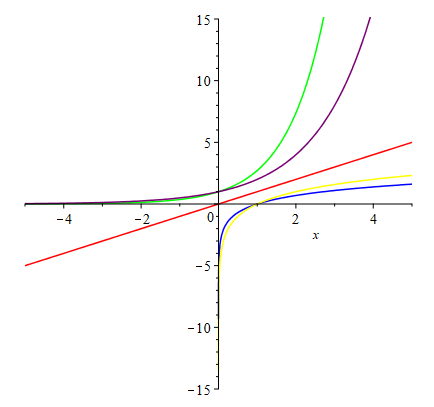
\includegraphics{figs/Log-Exp-Functions-01.png}
\caption{Graph of some logarithmic and exponential functions}
\end{figure}
\EndKnitrBlock{solution}

\BeginKnitrBlock{exercise}
\protect\hypertarget{exr:unnamed-chunk-3}{}{\label{exr:unnamed-chunk-3}
}Graph the following functions together. \[
y=\log_3x, \qquad y=3^x, \qquad y=(1/3)^x, \qquad y=\log_{1/3}x.
\]

Find the pairs that are symmetric to each other with respect to a
certain line.
\EndKnitrBlock{exercise}

\BeginKnitrBlock{exercise}
\protect\hypertarget{exr:unnamed-chunk-4}{}{\label{exr:unnamed-chunk-4}
}Graph the following functions together. \[
y=0.5^x, \qquad y=2^x, \qquad y=5^x.
\]

Describe the monotonicity (increasing/decreasing) of the functions?

Fix an input \(x\). Describe how \(y\)-values change when bases changes
from small number to bigger number?
\EndKnitrBlock{exercise}

\BeginKnitrBlock{exercise}
\protect\hypertarget{exr:unnamed-chunk-5}{}{\label{exr:unnamed-chunk-5}
}Graph the following functions together. \[
y=\log_{0.5}x, \qquad y=\log_2x, \qquad y=\log_{5}x.
\]

Describe the monotonicity (increasing/decreasing) of the functions?

Fix an input \(x\). Describe how \(y\)-values change when bases changes
from small number to bigger number?
\EndKnitrBlock{exercise}

\section{Differentiation and
integration}\label{differentiation-and-integration}

In Maple, one way to do differentiation and integration is to use the
\texttt{Calculus\ Palette} on the left side.

\begin{figure}
\centering
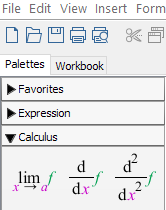
\includegraphics{figs/Calculus-Palette.png}
\caption{Calculus Palette in Maple}
\end{figure}

The other way is to use the commands \texttt{diff(f(x),\ x)} ,
\texttt{int(f(x),\ x)}, and \texttt{int(f(x),\ x=a..b)}.

Supported by the \texttt{Student{[}Calculus1{]}} package, Maple also
provides the tutor commands \texttt{DiffTutor()} and \texttt{IntTutor()}
which can show step-by-step solution of differentiation and integration.

Note you may also access tutor commands from the \texttt{Start} page
(click the home button in the toolbar and look for Calculus).

\BeginKnitrBlock{example}
\protect\hypertarget{exm:unnamed-chunk-6}{}{\label{exm:unnamed-chunk-6}
}Find \(y'\), where \(y=\ln \left(x^{3}+5x+1\right)\).
\EndKnitrBlock{example}

\BeginKnitrBlock{solution}
\iffalse{} {Solution. } \fi{} Using \texttt{diff}:

\begin{verbatim}
diff(ln(x^3+5*x+1), x)
\end{verbatim}

We get \[
y'=\dfrac{3x^{2}+5}{x^{3}+5 x+1}.
\]

Type in (assume that \texttt{with(Student{[}Calculus1{]})} was run)

\begin{verbatim}
DiffTutor(ln(x^3+5*x+1), x)
\end{verbatim}

and hit enter you will see

\begin{figure}
\centering
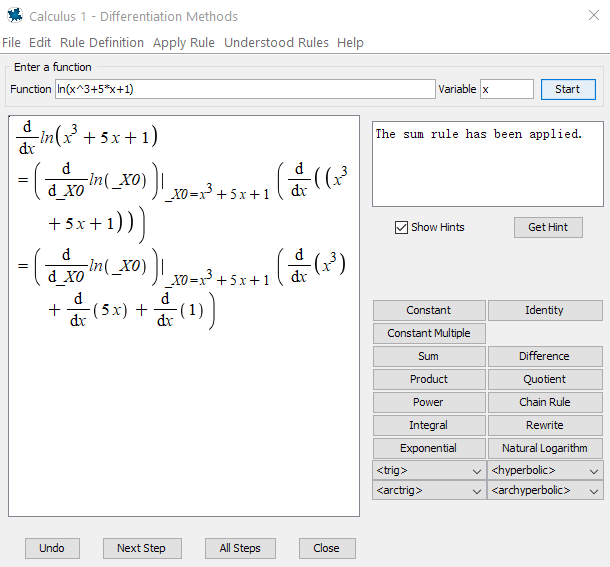
\includegraphics{figs/DiffTutor-ex.png}
\caption{}
\end{figure}

By click \texttt{Next\ Step} or \texttt{All\ Steps} you will see
detailed solution with rules used.
\EndKnitrBlock{solution}

\BeginKnitrBlock{example}
\protect\hypertarget{exm:unnamed-chunk-8}{}{\label{exm:unnamed-chunk-8}
}Evaluate the integral \[
\int\dfrac{e^x-1}{e^x+1}\mathrm{d} x.
\]
\EndKnitrBlock{example}

\BeginKnitrBlock{solution}
\iffalse{} {Solution. } \fi{} Using \texttt{int}:

\begin{verbatim}
int((exp(x)-1)/(exp(x)+1), x)
\end{verbatim}

We get \[
\int\dfrac{e^x-1}{e^x+1}\mathrm{d} x=2 \ln \left(\mathrm{e}^{x}+1\right)- x+C.
\]

Type in (assume that \texttt{with(Student{[}Calculus1{]})} was run)

\begin{verbatim}
IntTutor((exp(x)-1)/(exp(x)+1), x)
\end{verbatim}

and hit enter you will see

\begin{figure}
\centering
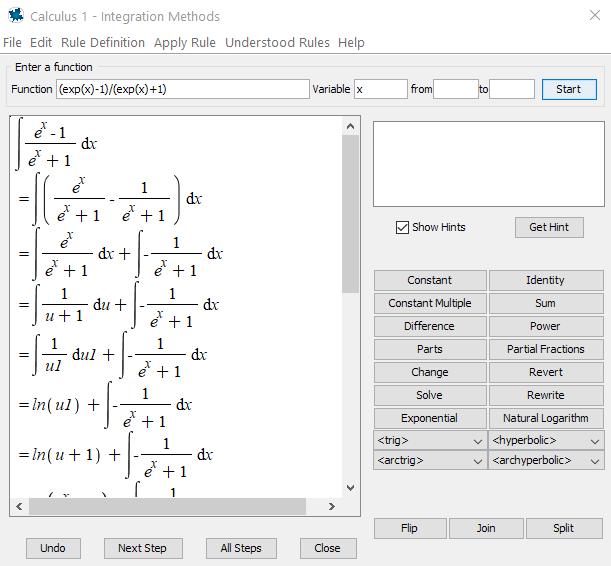
\includegraphics{figs/IntTutor-ex.png}
\caption{}
\end{figure}

By click \texttt{Next\ Step} or \texttt{All\ Steps} you will see
detailed solution with rules used.
\EndKnitrBlock{solution}

\BeginKnitrBlock{exercise}
\protect\hypertarget{exr:unnamed-chunk-10}{}{\label{exr:unnamed-chunk-10} }
Find the derivative \(\frac{\mathrm{d} y}{\mathrm{d} x}\), where
\(y=\ln|\cos x|\)
\EndKnitrBlock{exercise}

\BeginKnitrBlock{exercise}
\protect\hypertarget{exr:unnamed-chunk-11}{}{\label{exr:unnamed-chunk-11} }
Find the derivative \(\frac{\mathrm{d} y}{\mathrm{d} x}\), where
\(y=x^{\cos x}\)
\EndKnitrBlock{exercise}

\BeginKnitrBlock{exercise}
\protect\hypertarget{exr:unnamed-chunk-12}{}{\label{exr:unnamed-chunk-12} }
Evaluate the integral \[
\int \frac{\left(e^{4x}+e^{2x}\right)}{e^{3x}} d x
\]
\EndKnitrBlock{exercise}

\BeginKnitrBlock{exercise}
\protect\hypertarget{exr:unnamed-chunk-13}{}{\label{exr:unnamed-chunk-13} }
Evaluate the integral \[
\int 2^{3x} d x
\]
\EndKnitrBlock{exercise}

\chapter{Solve differential
equations}\label{solve-differential-equations}

In Maple, you may solve the equation \(y'(x)=k y(x) + c\) (which is
called an ODE) using the command \texttt{dsolve(\{ics,\ eq\})}, where
\texttt{ics} stands for initial condition \(y(0)=c\) and \texttt{eq}
stands for the differential equation. Without the \texttt{ics},
\texttt{dsolve} will provide a general solution.

\BeginKnitrBlock{example}
\protect\hypertarget{exm:unnamed-chunk-1}{}{\label{exm:unnamed-chunk-1}
}Find the function \(f(x)\) which satisfies the differential equation
\(f'(x)=k f(x)\) with \(f(0)=5\) and \(f(2)=3\).
\EndKnitrBlock{example}

\BeginKnitrBlock{solution}
\iffalse{} {Solution. } \fi{} Use the following command

\begin{verbatim}
dsolve({f(0)=5, f'(x)=k f(x)})
\end{verbatim}

we get \(f(x)=5e^{kx}\).

To find \(k\), we solve the equation \(3=5e^{2k}\) by

\begin{verbatim}
solve(3=5*e^(2*k), k)
\end{verbatim}

which shows that \(k=\frac{\ln3-\ln5}{2}\approx -0.255\). Here we use
\texttt{evalf(\%)} (\% represents the previous result) to get the
approximation.

So the function \(f\) is given by \[
f(x)=5e^{\frac{x(\ln3-\ln5)}{2}}\approx 5e^{-0.255x}.
\]
\EndKnitrBlock{solution}

\BeginKnitrBlock{exercise}
\protect\hypertarget{exr:unnamed-chunk-3}{}{\label{exr:unnamed-chunk-3} }
Find the function \(y\) which satisfies the differential equation
\(y'(x)=k y(x)\) with \(y(0)=2\) and \(y(5)=11\).
\EndKnitrBlock{exercise}


\end{document}
